\section{Zielsetzung}
\label{sec:Zielsetzung}
Unter anderem in technischen Anwendungen und in der Freizeit
(z.B. beim Tauchen oder Fallschirmspringen)
werden Unterdruck- oder Vakuumbereiche verwendet.
Dies motiviert eine genauere Betrachtung der Grundlagen der Vakuumtechnik
in diesem Versuch.
% In diesem Versuch werden die Grundlagen der Vakuumtechnik genauer betrachtet.
% Da die Technik und Freizeit (z.B. Tauchen oder Fallschirmspringen) ohne die Erforschung und Verwendung von Unterdruck- und Vakuumbereichen nicht vorzustellen
% ist, sollen in diesem Versuch die Grundlagen der Vakuumtechnik genauer betrachtet werden.
Genauer soll der Aufbau eines Pumpstandes zur Bestimmung von Evakuierungskurven und Leckratenmessungen
bei einer Drehschieberpumpe und einer Turbomolekularpumpe (im weiteren als TMP bezeichnet) verwendet werden.
Aus diesen Daten sollen dann das effektive Saugvermögen berechnet und gegen die Druckabhängigkeit dargestellt werden.


\section{Theorie}
\label{sec:Theorie}
\subsection{Grundbegriffe}

Im Folgenden werden zunächst die wichtigsten Begriffe der Vakuumphysik näher erläutert.
\paragraph{Vakuum:}
Die allgemeine Annahme, dass das Vakuum ein vollständig leerer Raum ist, ist nach Definition der
deutschen Industrienorm nicht korrekt.
Ein Vakuum ist dort definiert als
\enquote{der Zustand eines Gases, wenn in einem Behälter der
Druck des Gases und damit die Teilchenzahldichte niedriger ist als außerhalb oder wenn der Druck
des Gases niedriger ist als \SI{300}{\milli\bar},
d. h. kleiner als der niedrigste auf der Erdoberfläche vorkommende Atmosphärendruck} \cite{vakuum}.

Das Vakuum wird in einzelne Druckbereiche unterteilt,
die anhand der mittleren freien Weglänge der Teilchen charakterisiert werden.
% Das Vakuum kann in einzelne Druckbereiche unterteilt werden, die abhängig von der mittleren
% freien Weglänge der Teilchen sind.
Eine solche Unterteilung ist in Tabelle \ref{tab:Vakuum} zu finden.

\begin{table}
  \centering
  \caption{Druckbereiche mit konventionellem Namen, Teilchenzahldichte $n$ und mittlerer freier Weglänge $\lambda$.}
  \label{tab:Vakuum}
  \begin{tabular}{cccc}
    \toprule
    &$p$ in \si{\milli\bar} & $n$ in Teilchen/\si{\centi\raiseto{3}\meter} & $\lambda$ \\
    \midrule
    Umgebungsdruck & 1013 & \num{2.7e19} & \SI{68}{\nano\meter} \\
    Unterdruck & > 300 & > 10$^{19}$ & < \SI{0.1}{\micro\meter} \\
    Grobvakuum & 300 - 1 & 10$^{19}$ - 10$^{16}$ & \num{0.1} - \SI{100}{\micro\meter} \\
    Feinvakuum & 1 - 10$^{-3}$ & 10$^{16}$ - 10$^{13}$ & \num{0.1} - \SI{100}{\milli\meter} \\
    Hochvakuum & 10$^{-3}$ - 10$^{-7}$ & 10$^{13}$ - 10$^{9}$ & \SI{10}{\centi\meter} - \SI{1}{\kilo\meter} \\
    Ultrahochvakuum & 10$^{-7}$ - 10$^{-12}$ & 10$^{9}$ - 10$^{4}$ & \SI{1}{\kilo\meter} - 10$^5\,$\si{\kilo\meter} \\
  \end{tabular}
\end{table}

\paragraph{Druck und Partialdruck:}
\enquote{Der Druck ist definiert als der Betrag einer senkrecht und gleichmäßig auf eine Flächeneinheit wirkenden Kraft} \cite{pfeiffer}.
\begin{equation}
  p = \frac{F}{A}
\end{equation}
Da ein Gas wie z.B. Luft nicht nur aus einer Teilchensorte besteht und jede Sorte ihren eigenen Anteil zum Totaldruck darstellt, werden
die einzelnen entstehenden Teilrücke als Partialdrücke bezeichnet. Eine graphische Darstellung der Druckarten ist in \ref{fig:Druck} zu finden.
Dabei zeigt die linke Abbildung einen Gasbehälter mit einer einzelnen grün markierten Gasart,
welche einen Totaldruck erzeugt.
Die rechte Abbildung hingegen zeigt einen Gasbehälter mit unterschiedlichen
Teilchensorten in verschiedenen Farben, die jeweils einen mit $p_\text{p}$
gekennzeichneten Partialdruck erzeugen.

\begin{figure}
  \centering
  \begin{subfigure}[b]{0.49\textwidth}
    \centering
    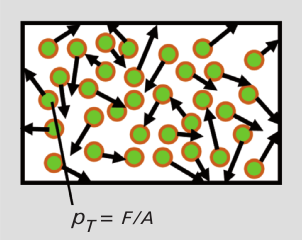
\includegraphics[width=0.5\textwidth]{Druck.png}
  \end{subfigure}
  \begin{subfigure}[b]{0.49\textwidth}
    \centering
    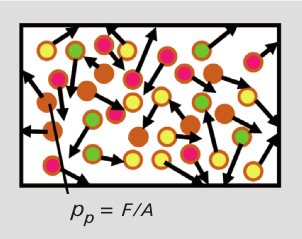
\includegraphics[width=0.5\textwidth]{Partialdruck.png}
  \end{subfigure}
  \caption{Graphische Darstellung von Druck und Partialdruck durch Impulse von Teilchen nach \cite{pfeiffer}.}
  \label{fig:Druck}
\end{figure}

\paragraph{Mittlere freie Weglänge:}
Die mittlere freie Weglänge $\lambda$ ist definiert als die durchschnittliche Weglänge, die
ein Teilchen zurücklegt, bis es zu einem Stoß mit einem anderen Teilchen kommt. Es gilt
\begin{equation}
  \lambda = \frac{1}{n\cdot\sigma}
  \label{eqn:Weglaenge}
\end{equation}
mit der Teilchenzahldichte $n$ und dem Wirkungsquerschnitt $\sigma$.
Unter Verwendung eines idealen Gases, bei dem sich die Teilchen nach der Maxwellschen Geschwindigkeitsverteilung
bewegen, gilt
\begin{equation}
  \lambda = \frac{k_\text{B}T}{\sqrt{2}\pi p d^2}
\end{equation}
mit der Boltzmann-Konstanten $k_\text{B}$, der Temperatur $T$,
dem Durchmesser des Moldeküls $d$ und dem Druck $p$.
% \begin{equation*}
%   \text{mit }k_\text{B}:\text{Boltzmann-Konstante }, T:\text{Temperatur}, d:\text{Durchmesser d. Moleküls }, p:\text{Druck}
% \end{equation*}
\paragraph{Ideales Gas:}
Das ideale Gas ist ein Modell aus der Thermodynamik, um Gas möglichst einfach beschreiben zu
können. Dabei wird davon ausgegangen, dass die Gasteilchen nur untereinander oder mit den Wänden
(innerhalb derer sich das entsprechende Gas befindet) elastisch stoßen.
Daraus lässt sich die ideale Gasgleichung
\begin{equation}
  p \cdot V = N \;k_\text{B}\;T
  \label{eqn:ideal}
\end{equation}
mit der Teilchenzahl $N$ und dem Volumen des Gefäßes $V$ folgern.
% \begin{equation*}
%   \text{mit }p:\text{Druck }, V:\text{Volumen d. Gefäßes }, N:\text{Teilchenzahl}
% \end{equation*}
% folgern.
Für konstante Temperaturen ergibt sich das Gesetz von Boyle-Mariotte
% Aus der Idealen Gasgleichung für $T\,$=$\,$const das Gesetz von Boyle-Mariotte, welches besagt,
% dass bei konstanter Temperatur der Zusammenhang
\begin{equation}
  p \sim V^{-1}.
\end{equation}
% gilt.

\paragraph{Stömungsarten:}
Bei der Unterscheidung von verschiedenen Strömungsarten ist die Knudson-Zahl
\begin{equation}
  K_\text{N} = \frac{\lambda}{l}
  \label{eqn:Knudsen}
\end{equation}
von Bedeutung.
Diese ist definiert als die mittlere freie Weglänge $\lambda$ pro charakteristischer Länge des
durchströmten Mediums $l$.
Dabei ist die charakteristische Länge die räumliche Breite des Mediums
senkrecht zur Strömungsrichtung.
% dies ist die Distanz im Mediums, die die Stömung durchquert und mit den
% Seiten wechselwirken kann..
Für eine Knudsen-Zahl zwischen \num{0.01} und \num{0.5} wird der Begriff Knudsenströmung verwendet.
Diese Knudsen-Strömung taucht besonders im Bereich des Feinvakuums auf,
welches oft in technischen Anwendungen verwendet wird.
Bei einer Knudsenzahl von $K_\text{N} < \num{0.01}$ wird von einer Kontinuumsströmung gesprochen,
die vor allem im Grobvakuum auftritt.
Im weiteren Verlauf werden die laminare und die turbulente Strömung betrachtet.
Gilt $K_\text{N} > \num{0.5}$, so ist die mittlere freie Weglänge wesentlich größer als die Abmessung des Strömungskanals
und es lassen sich kaum noch Wechselwirkungen mit anderen Gasteilchen feststellen.
Es kommt zur molekularen Strömung,
die vor allem im Bereich des Hoch- und Ultrahochvakuums aufzufinden ist.

\subsection{Vakuumtechnik:}
Bei der Unterscheidung von verschiedenen Typen von Vakuumpumpen kommt es auf die verschiedenen Arten der
Wechselwirkung zwischen Gasteilchen und Wänden an (vergleiche~\cite{pfeiffer}).

\paragraph{Sorption:}
Als Sorption bezeichnet man die Aufnahme eines Teilchens durch Ab- oder Adsorption
in einen Körper oder Stoff.

\paragraph{Absorption:}
Ein Atom, Molekül oder Ion wird vollständig im Körper oder Stoff aufgenommen.
% Ein Atom, Molekül oder Ion wird von einer anderen Phase vollständig
% aufgenommen.

\paragraph{Adsorption:}
Anders als bei der Absorption, wird das Atom, Molekül oder Ion hier nur auf der Oberfläche des Körpers
festgehalten und nicht komplett aufgenommen.

\paragraph{Desorption:}
Dies ist die Umkehrung der Sorption, also die Abgabe eines Atoms, Moleküls oder Ions.

\paragraph{Diffusion:}
Diffusion beschreibt den Ausgleich eines Konzentrationsgefälles zwischen
zwei Bereichen.
Dieser Ausgleich ermöglicht das Anlegen eines Vakuums im gesamten
Rezipienten, obwohl sich die Pumpe an einer festen Position befindet.
% Dies ist der Ausgleich zwischen zwei Bereichen verschiedener Konzentrationen
% aufgrund von Brownscher Molekularbewegung.
% In der Vakuumsphysik tritt dies auf, wenn es während des Anlegens eines
% Vakuums zu einem Gasdruckabfalls im Rezipienten kommt.

Da es auf der Erde kein natürliches Vakuum gibt, ist es unverzichtbar auf Vakuumpumpen zurückzugreifen.
Hier werden zwei Arten von Vakuumpumpen betrachtet:

\paragraph{Drehschieberpumpe (nach \cite{pfeiffer}):}
Die Drehschieberpumpe gehört zur Kategorie der Gastransferpumpen und besteht aus einem Gehäuse (auch Stator genannt),
einem exzentisch eingebautem Rotor und einem im Rotor eingebautem Schieber,
welcher durch eine Feder an das Gehäuse gedrückt wird.
Ein- und Ausgang des Gehäuses sind durch Ventile gesichert.
Dieser Aufbau ist in Abbildung \ref{fig:DSP} zu finden.
Der Schieber teilt den Arbeitsraum in Druck- und Saugbereich ein.
Fährt der Schieber an dem Einlassventil vorbei,
so liegt in diesem \enquote{neu} entstandenen Volumen nach Boyle-Mariotte
ein geringerer Druck als im Einlassventil vor und Gas strömt ein.
Nachdem der Einlass wieder geschlossen ist,
wird das Gas zwischen den zwei Scheiben komprimiert und nach
Boyle-Mariotte steigt der Druck.
Ist der Druck groß genug, so öffnet sich das Auslassventil (Federventil) und das Gas strömt heraus.
Während dieses Vorganges befindet sich immer etwas Öl im Arbeitsraum,
um den Schieber zu schmieren und den Raum abzudichten.

Diese Art von Vakuumpumpen wird bis zu einem Feinvakuum als Hauptpumpe verwendet.
Für geringere Drücke wird ein solches Gerät als Vorpumpe verwendet,
z.B. vor einer TMP.
% Bei einem Hochvakuum und geringeren Druckbereichen wird
% ein solches Gerät als Vorpumpe verwendet, z.B. vor einer TMP.

\begin{figure}
 \centering
 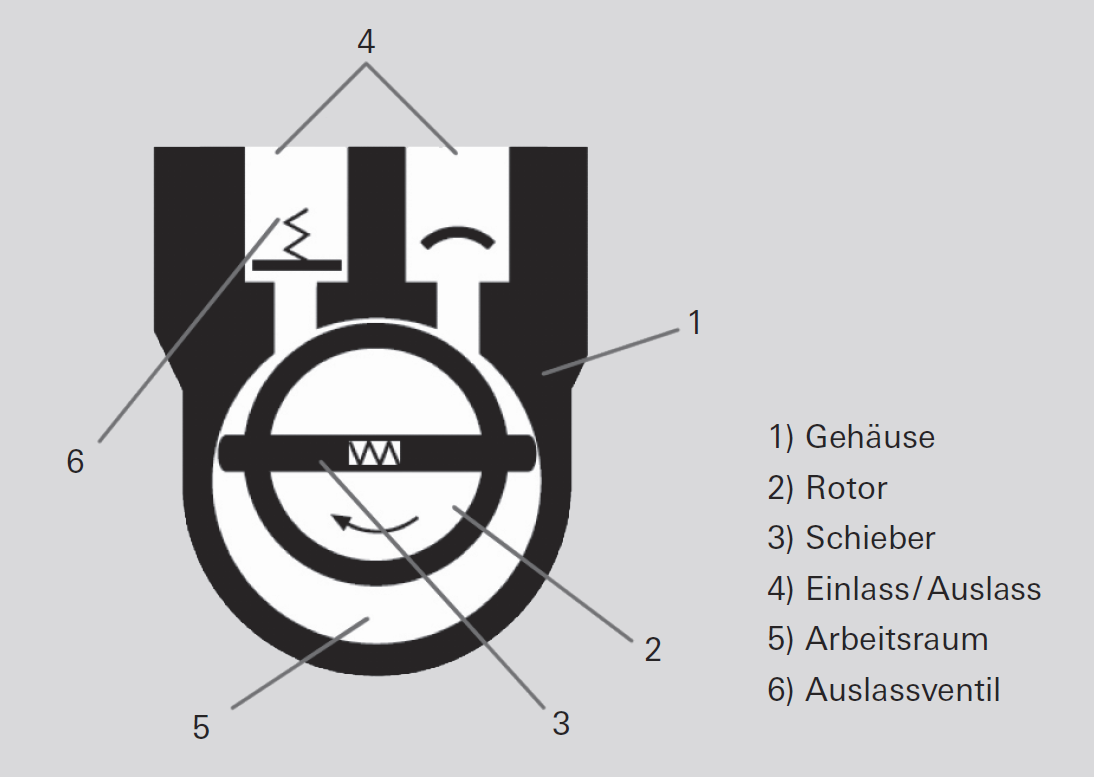
\includegraphics[width=0.5\textwidth]{Drehschieberpumpe.png}
 \caption{Schematische Darstellung einer Drehschieberpumpe \cite{DSP}.}
 \label{fig:DSP}
\end{figure}

\paragraph{Turbomolekularpumpe (nach \cite{pfeiffer}):}
Diese Art der Molekularpumpe besteht aus einer mehrstufigen Anordnung von Statoren und Rotoren
und benötigt ein Vorvakuum von ungefähr
\SI[retain-unity-mantissa=false]{1e-3}{\milli\bar},
sodass liegt eine molekulare Strömung vorliegt.
In Abbildung \ref{fig:TMP} ist der Aufbau schematisch dargestellt.
Die Rotoren drehen sich mit bis zu \SI{1500}{\hertz} und geben einfallenden
Teilchen einen zusätzlichen Impuls.
In der schematischen Darstellung fallen Teilchen von oben ein und erhalten
aufgrund einer Schräge der Rotoren einen Impuls nach unten.
Im Anschluss treffen sie auf die Statoren,
welche eine spiegelverkehrte Schräge aufweisen und eine Bewegung des Teilchens
nach unten verstärken.
Somit werden auf die Rotoren treffende Teilchen
in die Richtung der Vorvakuumpumpe beschleunigt.
Ein Vorvakuum ist bei dieser Pumpenart notwendig,
da die mittlere freie Weglänge größer sein muss als der Abstand der Rotorblätter.
Ansonsten käme es zwischen den Statoren und Rotoren zu Stößen der Teilchen untereinander,
sodass im Mittel keine Beschleunigung in Richtung der Vorvakuumpumpe erzeugt wird.
% Alte Beschreibung
% Dabei sollen die Rotoren den Gasteilchen einen zusätzlichen Impuls geben.
% Der sie dazu bringt, auf die Statoren zu treffen und abtransportiert zu werden.
% Dafür muss im Rezipienten selbst eine molekulare Strömung vorliegen.
% Die freie mittlere Weglänge muss zudem größer sein als der Abstand der Rotorblätter.
% Daher muss das Vakuum im Rezipienten schon vor dem Einschalten der TMP bei ca.
% \SI[retain-unity-mantissa=false]{1e-3}{\milli\bar} liegen.
% Ansonsten würden die Teilchen zwischen den Statoren und Rotoren stoßen
% und wieder in den Rezipienten gelangen,
% somit würde kein höheres Vakuum erreicht werden können.
% Dieser Aufbau ist in Abbildung \ref{fig:TMP} graphisch dargestellt.
\begin{figure}
  \centering
  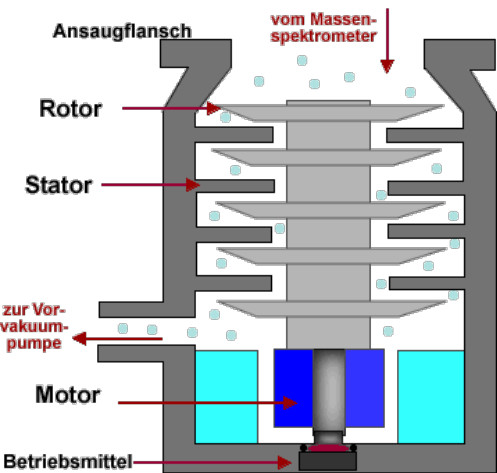
\includegraphics[width=0.4\textwidth]{TMP.JPG}
  \caption{Schematische Darstellung einer Turbomolekularpumpe \cite{TMP}.}
  \label{fig:TMP}
\end{figure}
\FloatBarrier

\paragraph{Saugvermögen:}
Zur Bestimmung des Saugvermögens $S$ (geförderter Volumenstrom) müssen folgende theoretische Annahmen getroffen werden \cite{anleitung}:
\begin{enumerate}
 \item Es gilt während der gesamten Messung $\dot{V} = const$.
 \item Das verwendete Gas kann als ideales Gas angenommen werden.
 \item Die Messungen werden bei $T = const$ getätigt.
 \item Das Gas ist zu jedem Zeitpunkt im thermischen Gleichgewicht.
 \item Lecks und Effekte der Desorption sind zu vernachlässigen.
 \item Das Saugvermögen $S$ ist konstant und unabhängig vom Druck.
\end{enumerate}
Wird die ideale Gasgleichung nach der Zeit abgeleitet und die Relation $\dot{V} = S = const$ eingesetzt,
so folgt die Gleichung
\begin{equation}
  \dot{p}V = -pS.
\end{equation}
Die so entstandene Differentialgleichung lässt sich durch den Exponentialansatz
\begin{equation}
  p(t) = p_0 \text{e}^{-\frac{t}{\tau}}
\end{equation}
lösen. Dabei ist $p_0$ ein gegebener Anfangsdruck. Durch Einsetzen ergibt sich
\begin{equation}
  \tau = \frac{V}{S}
\end{equation}
Wird nun ein endlicher Enddruck $p_\text{E}$ berücksichtigt, so folgt die Gleichung
\begin{equation}
  p(t) = (p_0 - p_\text{E})\text{e}^{-\frac{tS}{V}}+p_\text{E}.
  \label{eqn:druck}
\end{equation}
Der Einsatz eines Enddrucks folgt aus Effekten wie der Desorption,
sowie realer und virtueller Lecks.
Virtuelle Lecks stehen dabei für die Diffusion von Teilchen durch die
Rezipientenwand in das Vakuum.
Durch die Funktionsweise einer Pumpe kann nur ein endlicher Enddruck erreicht werden,
da Effekte wie ein vorhandenes
Totvolumen sowie ein endliches Kompressionsvermögen vorliegen können.

\paragraph{Leckrate:}
Um zu ermitteln, wieviel Gas pro Zeit aus dem Aufbau geleckt ist, wird die Leckrate $Q$ durch
\begin{equation}
  S  = \frac{Q}{P_\text{G}} \text{ mit } Q = V\,\frac{\symup{d} p}{\symup{d} t}
\end{equation}
defininiert. Daraus folgt das Saugvermögen
\begin{equation}
  S = \frac{V}{p_\text{G}}\frac{\symup{d} p}{\symup{d} t}.
  \label{eqn:Saug}
\end{equation}

\paragraph{Leitwerte:}
Durch verschiedene Phänomene wie Strömungswiderstände der Verbindungsstücke
lässt sich das vom Hersteller angegebene Saugvermögen $S_0$ nicht erreichen.
Daher wird ein effektives Saugvermögen $S_\text{eff}$ oder \enquote{Nennsaugvermögen} von
\begin{equation}
   \frac{1}{S_\text{eff}} = \frac{1}{S_0} + \frac{1}{L}
   \label{eqn:effSaug}
\end{equation}
erwartet.
Dabei ist $L$ der Leitwert, welcher den reziproken Strömungswiderstand darstellt.
% TODO erläutern, wovon der Leitwert abhängt. Dabei auf Strömungsarten
% und Geometrie des Rohres eingehen.

\paragraph{Leck:}
Als ein Leck wird eine undichte Stelle innerhalb eines Rezipienten bezeichnet,
durch welches Teilchen aus dem System entweichen oder eindringen.
In der Vakuummphysik wird zwischen realen und virtuellen Lecks unterschieden.
Reale Lecks sind physische Löcher im Aufbau,
wohingegen virtuelle Lecks Desorptions- oder Diffusionsprozesse von Teilchen an der
Rezipientenwand beschreiben.
Trotzdem verfälschen diese Effekte die Messwerte,
daher werden durch Erhitzen des Reizpienten (Ausheizen)
oder kurzzeitiges Befüllen mit Stickstoff (Fluten) die Desorptionsraten so weit es geht gesenkt.

Zur Messung des Drucks während der Messreihen werden 2 verschiedene Vakuummeter verwendet,
dabei hat jedes seinen eigenen Anwendungsbereich:

\paragraph{Pirani-Messgerät:}
Für hohe Druckbereiche ($p > \SI{10e-4}{\milli\bar}$) wird ein Pirani-Messgerät verwendet.
Dieses bestimmt den Druck des Gases über dessen Wärmeleitfähigkeit.
Diese sinkt bei kleinerem Gasdruck und die Temperatur des im Messgerät befestigten Glühdrahts steigt.
Wird der Glühdraht auf einer konstanten Temperatur gehalten,
so ändert sich mit der Wärmeleitfähigeit des Gases auch die benötigte messbare Heizleistung.
Wird dieses Messgerät in einem zu hohen Druckbereich verwendet,
so wird die Wärmleitung von der Konvektion überdeckt.
Bei zu niedrigen Drücken dominiert die Wärmestrahlung
und der eigentlich zu messende Effekt (Wärmeleitung) tritt in den Hintergrund.
Zudem tritt Wärmeleitung über die Aufhängung des Drahtes auf.

\paragraph{Glüh- und Kaltkathoden Vakuummeter:}
Bei einem Glühkathoden Vakuummeter werden die Elektronen durch
thermische Elektronenemission von der Kathode gelöst und die Gasteilchen durch Stöße ionisiert.
Die Anode ist zylindrisch und gitterförmig angeordnet,
in ihrer Mitte befindet sich ein als Auffänger dienender Draht,
welcher die Ionen aufsammelt.
Dieser resultierende Ionisationsstrom zwischen Anode und dem Aufhänger ist ein Maß für den Druck.
Die Funktionsweise des Kaltkathoden Vakuummeters ist nahezu analog zu der des Glühkathoden Vakuummeters,
nur werden die Elektronen nicht durch die thermische Elektronenemission,
sondern durch ein starkes äußeres elektrisches Feld aus der Kathode herausgelöst
(elektrische Feldemission).
